\documentclass[norsk,a4paper,12pt]{article}
\usepackage[utf8]{inputenc}
\usepackage{graphicx} %for å inkludere grafikk
\usepackage{verbatim} %for å inkludere filer med tegn LaTeX ikke liker
\usepackage{tabularx}
\usepackage{booktabs}
\usepackage{amsmath}
\usepackage{float}
\usepackage{color}
\usepackage{listings}
\usepackage{hyperref}
\usepackage{amsmath}
\usepackage{tikz}

\lstset{language=c++}
\lstset{basicstyle=\small}
\lstset{backgroundcolor=\color{white}}
\lstset{frame=single}
\lstset{stringstyle=\ttfamily}
\lstset{keywordstyle=\color{red}\bfseries}
\lstset{commentstyle=\itshape\color{blue}}
\lstset{showspaces=false}
\lstset{showstringspaces=false}
\lstset{showtabs=false}
\lstset{breaklines}
\lstset{postbreak=\raisebox{0ex}[0ex][0ex]{\ensuremath{\color{red}\hookrightarrow\space}}}
\usepackage{titlesec}

\setcounter{secnumdepth}{4}
\usetikzlibrary{through,calc,er,positioning}

\titleformat{\paragraph}
{\normalfont\normalsize\bfseries}{\theparagraph}{1em}{}
\titlespacing*{\paragraph}
{0pt}{3.25ex plus 1ex minus .2ex}{1.5ex plus .2ex}


\title{FYS4411 - Computational Physics II\\\vspace{2mm} \Large{Project 2}}
\author{\large Dorthea Gjestvang\\ Even Marius Nordhagen}
\date\today
\begin{document}

\maketitle

\begin{itemize}
\item Github repository containing programs and results: \\\url{https://github.com/evenmn/FYS4411/tree/master/Project%202}
\end{itemize}

\begin{abstract}
Abstract
\par 

\end{abstract}

\newpage

\tableofcontents

\newpage

\section{Introduction} \label{sec:Introduction}


\section{Theory} \label{sec:Theory}
\subsection{Presentation of potential} \label{sec:Presentation_of_potential}
In this project, we simulate a system of $P$ electrons trapped in a harmonic oscillator potential, with a Hamiltonian given by

\begin{equation}
\label{eq:Hamiltonian}
\hat{H} = \sum_{i=1}^{P} (-\frac{1}{2} \nabla_i^2 + \frac{1}{2} \omega^2 r_i ^2) + \sum_{i<j} \frac{1}{r_{ij}} 
\end{equation}

where $\omega$ is the harmonic oscillator potential and  $r_i = \sqrt{x_i^2 + y_i^2}$ is the position of electron $i$. The term $\frac{1}{r_{ij}}$ is the interacting term, where $r_{ij} = |r_i - r_j|$ is the distance between a given pair of interacting electrons. Natural units have been used, such that $\hbar = c = m_e = e = 1$.

Since electrons are fermions, we need an antisymmetric wavefunction under exchange of two coordinates, and we need to take the Pauli principle into account. A Slater determinant is therefore needed for multiple fermions to ensure that the total wavefunction is antisymmetric. In this project we will study particles in the ground state only, and according to the Pauli principle we can in this case study a maximum of two particles with spin $s=\pm 1/2$. The slater determinant for two particles read
\begin{equation}
\Psi_T=
\begin{vmatrix}
\Phi_1(\boldsymbol{r}_1) & \Phi_2(\boldsymbol{r}_1)\\
\Phi_1(\boldsymbol{r}_2) & \Phi_2(\boldsymbol{r}_2)
\end{vmatrix}
=\Phi_1(\boldsymbol{r}_1)\Phi_2(\boldsymbol{r}_2)-\Phi_2(\boldsymbol{r}_1)\Phi_1(\boldsymbol{r}_2)
\end{equation}
where $\Phi_i(\boldsymbol{r})$ is the single particle wave function (SPF) of state $i$. This contains a spatial part and a spin part, and we assume that it can be splitted up such that the spin part takes the antisymmetry property and does not affect the energy. Therefore we only need a symmetric spatial part to calculate the energies.

\subsection{Solving this with machine learning}
When solving a system of particles as the one described in the previous system with Variational Monte Carlo, as described in \cite{Nordhagen}, we would need an anzats for the wave function, where we use our physical intuition to create the form of a wave function with different variational parameters, and then let it be up to the computer to find the optimal parameters through a minimization method. However, this method is only as good as the physical intuition; if the form of the wave function is unrealistic, the results will be the same
\par 
\vspace{3mm}
This challenge can be mended by using machine learning. There are several different types of machine learning systems, and the one we will present and utilize in this project has the ability to learn and sample from a probability distribution. This is perfect for quantum mechanical problems, as we know from quantum mechanics the wave function $\Psi$ is nothing more than a probability denisty, giving that $\Psi^2$ is a probability distribution that says something about where a given particle most probabliy can be found. As we are solely interested in the energy of the two-fermion system, and not the exact wave function, the fact that the machine learning program does not explicitly give the wave function is therefore of no consequence. We still have to give some guidelines for the form of the probability distribution, but the machine learning program can sample from a larger variety of probability distributions compared to the form used in VMC.

\subsubsection{Machine learning}
With the goal of solving the quantum mechanical system presented in section \ref{sec:Presentation_of_potential} in mind, we should start by explaining what machine learning is. Machine learning is the idea that a computer can be trained to learn to yield certaint outputs, without directly being told exactly what to give. Examples on this is pattern recognizion, where the computer first is shown for example pictures of wolves and huskies. After training the computer on pictures where the computer sees huskies and wolves and is told the correct answer, it should after a sufficiently long training period, be able to recognize huskies and wolves by itself. 
\par 
\vspace{3mm}
The example described above is what we call supervised learning, where the correct output answer is known during the training program. A machine learning program could also be unsupervised, where the correct answer is unknown, or based on reinforcement learning, where the the program learns by conducting trial-and-error experiments. 
\par 
\vspace{3mm}

\subsubsection{Neural network}

 This sound amazing, and maybe even impossible. Therefore the question now is: how to program computers to learn, just like humans? The answer is, fittingly, that we should make the program run like the the human brain by implementing what is called a neural network. Inspired by neurons in the human brain, a neural network is a programmed network of variables, called nodes, that comminucate in a given manner. Each node preforms a simple process: based on the input it receives, and how that input is weighted, it decides wheter or not to fire. The mathematical model of an example of a neural node was presented by McCulloch and Pitts in 1943 \cite{Marsland}, shown in figure \ref{fig:neuron}, where the input is mared $x_i$, the weights deciding how much the input should count is $W_i$, and the output from the node based on $x_i$ and $W_i$ is called h. 

 \begin{figure} [H]
 	\centering
 	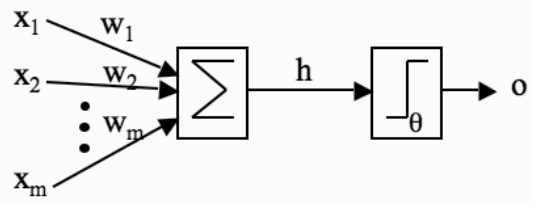
\includegraphics[scale=0.6]{plots/neuron.png}
 	\caption{McCullochs and Pitts' model of neutrons visualized. Image reproduced from \cite{Marsland} }
 	\label{fig:neuron}
 \end{figure}

The neutrons are arranged in layers in the neural network, one visible layer that receives the input, and up to several hidden layers. The layers are arranged such that the output values from the visible nodes is the input values of the visible nodes. The nodes can also have bias values, that shift the output value $h$ with a ceirtan number, and the nodes in different layers can be connected in different ways.  An example of a neural network with two layers is shown in figure \ref{fig:neural_network}.

 \begin{figure} [H]
	\centering
	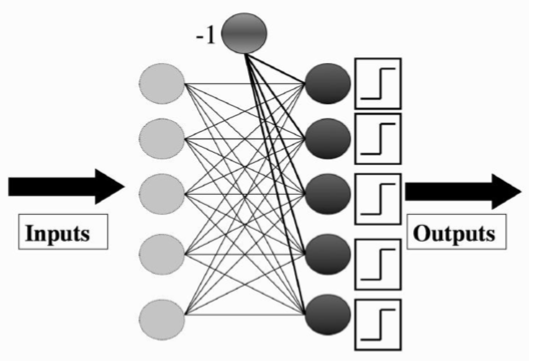
\includegraphics[scale=0.5]{plots/neural_network.png}
	\caption{An example of a neural network with one visible and one hidden layer of nodes, and with bias $-1$ on the hidden nodes. Image reproduced from \cite{Marsland} }
	\label{fig:neural_network}
\end{figure}

The idea behind machine learning is that the weights $W_i$, that decides how much a node puts emphazis on a given input, can be changed, and thus change the system's response to the same input. We will explain with the example from earlier, with huskies and the wolves: first, the program are shown pictures of wolves and huskies, and it is told the correct answer. The weights $W_i$ are then updated such that when a husky is shown, the output "husky" is generated, and the same for wolves. After a sufficiently long training period, the program's weights are optimalized for recognizing wolves and huskies. When shown a picture, the program should then by itself be able to determine wheter it is a wolf or a husky that it sees. 

\subsubsection{Restricted Boltzmann Machines}
There are plenty of ways to put together a neural network, as one can modify the number of nodes and layers, the bias, and also which nodes that are allowed to communicated. In this project, we will be using the so-called Restricted Boltzmann Machine (RBM). It is a two-layer network. The reason why it is named "restrictive" is that there are no connections between nodes in the same layer, but every node in the previous layer is connected to all the nodes in the next layer. The RBM can learn to draw samples from a probability distribution, which is just what we want in our project. In addition, we want to use a Gaussian-Binary RBM, where the hidden nodes have binary values, while the positions of the particles can take continous values, as they are, in fact, positions. 

The joint probability distribution is known from statistical mechanics,
\begin{equation}
F(\boldsymbol{X},\boldsymbol{H})=\frac{1}{Z}e^{-\beta E(\boldsymbol{X},\boldsymbol{H})}
\end{equation}
where we set $\beta=1/kT=1$ and $Z$ is the partition function, which can be ignored since it will vanish anyway. 

The system energy of a Gaussian-Binary RBM is given by
\begin{equation}
E(\boldsymbol{X},\boldsymbol{H})=\sum_{i=1}^{M}\frac{(X_i-a_i)^2}{2\sigma_i^2}-\sum_{j=1}^Nb_jH_j-\sum_{i,j=1}^{M,N}\frac{X_iW_{ij}H_j}{\sigma_i^2}
\end{equation}
(Hinton 2010). 

By setting $\Psi = F(\boldsymbol{X},\boldsymbol{H})$, we know have a general form of the probability distribution. In equation \ref{label} the form of the wave function is shown, when we have used that we have $M$ visible nodes and $N$ hidden nodes, and that the hidden nodes should take binary values. 

\begin{equation}
	\Psi = \frac{1}{Z} e^{\sum_i^M \frac{(X_i - a_i)^2}{2\sigma^2}} \prod_j^N (1+ e^{b_j + \sum_iM \frac{X_i W_{ij}}{\sigma^2}})
\end{equation}

\subsection{Energy calculation}



\subsection{Onebody density}

\subsection{Scaling}

\subsection{Error estimation}

\section{Method}

\subsection{Variational Monte Carlo}
\subsection{Metropolis Algorithm}
\subsubsection{Brute force}
\subsubsection{Importance sampling}
\subsubsection{Gibbs sampling}

\subsection{Gradient descent}
We use stochastic gradient descent to update the weights in order to minimize the local energy. The process itself is quite similar to that one typically used in Variational Monte Carlo (VMC) where the weights are our variational parameters, but compared with a normal VMC we have a lot more parameters to vary. The updating algorithm for updating the variational parameter $\alpha_i$ goes as
\begin{equation}
\alpha_i^+=\alpha_i-\eta d\alpha_i
\end{equation}
where the gradient of the local energy with respect to parameter $\alpha_i$ is
\begin{equation}
d\alpha_i=\frac{\partial\langle E_L\rangle}{\partial \alpha_i}=2\bigg(\Big\langle E_L\frac{1}{\Psi}\frac{\partial\Psi}{\partial\alpha_i}\Big\rangle-\Big\langle E_L\Big\rangle\Big\langle\frac{1}{\Psi}\frac{\partial\Psi}{\partial\alpha_i}\Big\rangle\bigg)
\end{equation}
where $\eta$ is the learning rate. We need to do this for all the parameters, and for our purposes it is convenient to vectorize the gradient such that $d\boldsymbol{a}$ and $d\boldsymbol{b}$ are vectors and $d\boldsymbol{W}$ is a matrix. The gradients to implement are
\begin{equation}
d\boldsymbol{a}=\frac{1}{\Psi}\frac{\partial\Psi}{\partial\boldsymbol{a}}=\frac{\boldsymbol{X}-\boldsymbol{a}}{\sigma^2}
\end{equation}
\begin{equation}
d\boldsymbol{b}=\frac{1}{\Psi}\frac{\partial\Psi}{\partial\boldsymbol{b}}=
\end{equation}

\subsubsection{Adaptive stochastic gradient descent}
A problem with the standard stochastic gradient descent method is that it will either converge fast, but the precision is poor, or the precision is good, but it converges slowly. To avoid this problem, we want a large learning rate when the energy is far from converging and a small learning rate when the energy converges. 

\section{Code}
\subsection{Structure}
\subsection{Implementation}

\section{Results} \label{sec:Results}

\section{Discussion} \label{sec:Discussion}

\section{Conclusion} \label{sec:Conclusion}

\newpage

\section{Appendix A - Local energy calculations} \label{sec:appendix_A}
The energy can be calculated by introducing a local energy, where the acerage local energy goes to the true energy with a sufficient amount of samples. This local energy can be splitted up in a kinetic part, a part from the harmonic oscillator potential and a interacting part,
\begin{equation}
E_L=\sum_{k=1}^{M}(E_{\text{KIN},k} + E_{\text{EXT},k})+E_{\text{POT}}.
\end{equation}
As discussed in \cite{Nordhagen}, the kinetic part can be expressed as
\begin{align}
E_{\text{KIN},k}&=\frac{1}{\Psi_T}\nabla_k^2\Psi_T\\
&=(\nabla_k\ln\Psi_T)^2+\nabla_k^2\ln\Psi_T
\end{align}
where we have used that
\begin{equation}
\frac{1}{\Psi_T}\nabla_k\Psi_T=\nabla_k\ln\Psi_T.
\end{equation}

\begin{equation}
\frac{\partial}{\partial X_k}\ln\Psi_T=-\frac{X_k-a_k}{\sigma^2}+\sum_{j=1}^{N}\frac{W_{kj}}{\sigma^2}\text{Logistic}(v(j))
\end{equation}
\begin{equation}
\frac{\partial^2}{\partial X_k^2}\ln\Psi_T=-\frac{1}{\sigma^2}+\sum_{j=1}^{N}\frac{W_{kj}^2}{\sigma^4}\text{Logistic}^2(v(j))e^{v(j)}
\end{equation}
where 
\begin{equation}
\text{Logistic}(x)=\frac{1}{1+e^x}
\end{equation}
and
\begin{equation}
v(j)=b_j+\sum_{i=1}^{M}\frac{X_iW_{ij}}{\sigma^2}.
\end{equation}
Thus the local energy can be expressed as
\begin{align}
E_L&=\sum_{i=1}^{N}\frac{\boldsymbol{W}_{*i}^T\boldsymbol{W}_{*i}}{\sigma^4}\text{Logistic}^2\big(v(i)\big)+\\
&\phantom{=}\sum_{i,j=1}^{N,N}\frac{\boldsymbol{W}_{*i}^T\boldsymbol{W}_{*j}}{\sigma^4}\text{Logistic}\big(v(i)\big)\text{Logistic}\big(v(j)\big)-\\
&\phantom{=}2\sum_{i=1}^N\frac{\boldsymbol{W}_{*i}^T(\boldsymbol{X}-\boldsymbol{a})}{\sigma^4}\text{Logistic}(v(i))+\\
&\phantom{=}\frac{(\boldsymbol{X}-\boldsymbol{a})^T\cdot(\boldsymbol{X}-\boldsymbol{a})}{\sigma^4}-\frac{1}{\sigma^2}+\boldsymbol{X}^T\boldsymbol{X}+E_{\text{INT}}
\end{align}



\newpage
\section{References}

\textcolor{red}{INCLUDE ONLY THOSE REFERENSES WE USE}

\begingroup
\renewcommand{\section}[2]{}
\begin{thebibliography}{}
	\bibitem{MHJ15}
	Morten Hjorth-Jensen.
	Computational Physics 2: Variational Monte Carlo methods, Lecture Notes Spring 2018.
	Department of Physics, University of Oslo,
	(2018).
	\bibitem{Marsland}
	S. Marsland, \emph{Machine Learning: An algorithmic Perspective, Second edition} (2015)
	\bibitem{Nordhagen}
	 D. Gjestvang, E. M. Nordhagen \emph{Computational Physics II: Project 1} (2018)
	
	
\end{thebibliography}
\endgroup

\end{document}
